% Section 1 (restructure plan, part 2). Every number is a macro of a generated numbers.tex (\fv: evidence_ledger_fresh.md;
% \nrv: evidence_ledger_natural_run.md; \plv, \dv: evidence_ledger_pilot.md, evidence_ledger_design.md). The scope of
% the evidence is stated once here (How far the evidence goes) and once in Section sec:threats.
\section{Introduction}
\label{sec:intro}
Executable tasks rebuilt from recorded agent sessions come from real use rather than curated issue trackers, and their verifiers can supply training rewards. Recent work reconstructs tasks and environments from interaction traces \cite{trace2eval}, curates executable tasks from developer--agent sessions \cite{swetogether,lu2026harvesting}, and releases large collections of such sessions \cite{swechat}. A session, however, is not a specification: users push back on what the agent did \cite{swechat}, and a reconstruction that keeps only the first request, or summarises the session without tracking which requirement each turn introduced, superseded or left open, can yield a verifier that rewards what the user rejected. An industry essay names this risk without measuring it \cite{guo2026production}.

We ask a conditional question: given a correction that adds or retracts requirements, does a verifier built without it accept violations of it, and do correction-aware reconstruction and a predefined audit avoid that without rejecting valid work? A \emph{task family} is a recorded session and everything derived from it. An agent receives a first request ($U_1$), its workspace is captured (the \emph{pre-correction state}), a correction ($U_2$) follows, and the agent's final state is the \emph{reference}. A \emph{contract} lists requirements, each with a status (explicit, inferred, superseded or unresolved) and evidence quotes from the session. The same frozen procedure generates verifiers from an \emph{initial-only} contract (recovered from $U_1$ alone) and a \emph{correction-aware} contract (from the whole session), each without and with a predefined \emph{audit} that grades audit candidates and lets a reviser change the tests (C1, C2 and C3, C4; Figure~\ref{fig:design}a). The audit's attacks come from the verifier's own contract, so it cannot supply a requirement the contract lacks, though a revision can tighten checks on behaviour the contract leaves open. We compare these with the repository's tests at the reference state (B1), which include tests the session agent added, and with a \emph{session-LLM baseline} (B2) that writes tests from the whole transcript without a contract. Fresh agents then attempt each task given the \emph{first request} alone or \emph{with the correction}. An attempt is \emph{invalid} if a model-written reference check, or a test of the base commit's suite that passes on the reference (the \emph{regression norm}), fails on it. False acceptance (FA) is the share of invalid attempts that a verifier passes, false rejection (FR) the share of valid attempts that it fails, and a \emph{reference gate} keeps a verifier only where it passes its own reference.

\IfFileExists{generated/figures/design_example.tex}{% Generated by `python paper/make_figures.py`; do not edit. Every value: paper/evidence_ledger_figures.md.
\begin{figure}[t]\centering
\ifdefined\includegraphics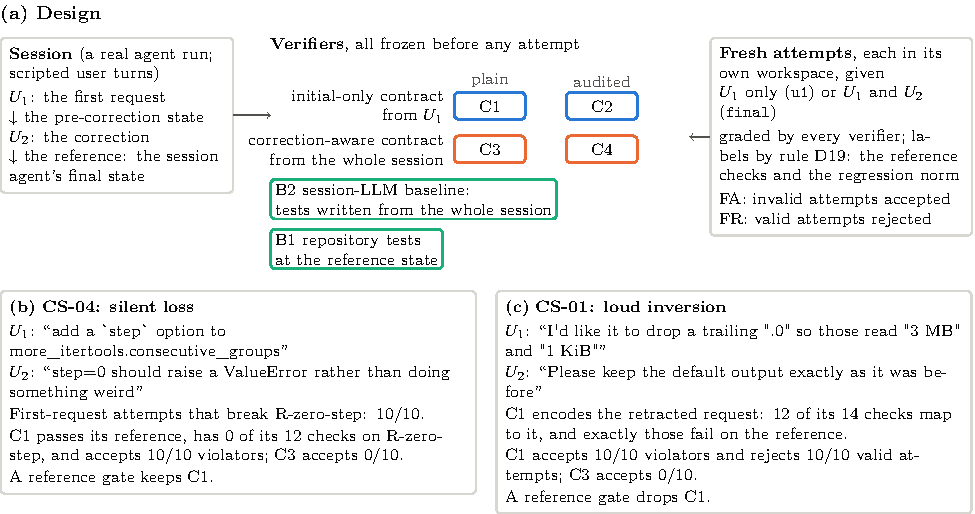
\includegraphics[width=\linewidth]{generated/figures/design_example.pdf}%
\else\unfilled{figure design\_example: main.tex must load graphicx}\fi
\caption{The design (a), and two worked examples from the fresh-agent stratum, run \texttt{fresh-v1}, under rule D19's labels and read post hoc: (b) CS-04 and (c) CS-01, each with excerpts of its first request ($U_1$) and correction ($U_2$), quoted from the synthetic scenario files. Every number in the panels is a value of Tables~\ref{tab:fresh-family}, \ref{tab:fresh-behaviours} and~\ref{tab:fresh-cv}. $^{\diamond}$Automated pilot; model-proposed labels, no human labels; 4 controlled families; descriptive (\S\ref{sec:intro}).}\label{fig:design}
\end{figure}
}{\unfilled{figure design\_example (make\_figures.py)}}

\paragraph{Findings.} Every analysed attempt that saw the correction is valid (\fv{solve.final}; \fv{attempts.excluded.w} attempt was excluded after its audit). Of the \fv{cv.attempts} that saw only the first request, \fv{u1.invalid.n} are invalid: \fv{cv.n} violate a requirement the correction introduced, and \fv{unspec.n} only break a base-commit test that the reference passes (the regression norm). The planned measure (protocol~\S15.4, estimand~3) is how C1 and C3 grade the violators: C1 accepts \fv{cv.c1}, C3 \fv{cv.c3} (\S\ref{sec:results-controlled}). Read post hoc, by behaviour, the violators show a \emph{silent loss} and a \emph{loud inversion}. In CS-03 and CS-04 the correction only adds requirements; C1 passes its reference, so a reference gate keeps it, yet it accepts \fv{cv.silent.c1} violators there (C3: \fv{cv.silent.c3}), and none of its checks maps to the requirement they break. In CS-01 the correction retracts a requirement of the first request; C1 encodes the retracted request and fails its own reference, which a gate would catch. CS-02 has no correction violator. Repository tests at the reference state cut both ways: they reject \fv{b1.fr} valid attempts, all through the tests the session agent added, and without those tests they accept \fv{b1.base.fa} invalid ones. In the natural case studies (\S\ref{sec:natural-cases}), the pre-review state, the tree a reviewer commented on and so invalid with respect to the correction under the source-evidence label, was rejected by C1 to C4 and B2 in NP-03, NP-04, NP-05, NP-18, NP-19 and NP-20; B1 accepted it in NP-03, NP-05, NP-19 and NP-20, where B1 equals the regression norm or part of it, and B3, a secondary diff-derived arm, in NP-04.

Our working hypothesis was that verifiers built from a session's final requirements, with evidence links and an audit, accept fewer violators than verifiers built from the first request. The data are consistent with the hypothesis, descriptively, for correction-aware against initial-only reconstruction on these \fv{families.w} tasks. They show no benefit of the audit, which added false rejections (C4 \fv{c4.fr} against C3 \fv{c3.fr}). On false acceptance, structured contracts did not differ from a session-LLM baseline.

\paragraph{How far the evidence goes.} This is an automated pilot: every label is a model proposal; no human label exists. Every model-written artifact comes from models of one model family of one provider, which are not named. The \fv{families.w} tasks were written by the study's own agent, and the fresh attempts add candidates, not tasks: they reuse the tasks and frozen verifiers of an earlier construction pilot (\S\ref{sec:pilot}) and were designed after its results were known. The silent-loss subset is a post hoc reading of the secondary, reference-gated view. No family-level sign-flip test over \fv{families.w} families can go below one-sided $p=\fv{cmp.floor.one}$, so every result is descriptive, and the design cannot say how often corrections are lost in practice. The natural arm, in which a reviewer's comment on an agent's pull request plays the correction, is reported as \nrv{families} exploratory case studies, family by family (\S\ref{sec:natural-cases}).

\paragraph{Contributions.} Prior work builds tasks from sessions and measures verifier errors (\S\ref{sec:related}); what we add is narrow. (a)~Withholding the correction from fresh agents, as a source of agent-made negatives that no generator wrote. (b)~How verifiers built with and without the correction grade those violators, with nulls for the audit and for structured contracts against a session-LLM baseline. (c)~The double edge of agent-added tests in repository suites taken at the reference state. (d)~Infrastructure, not a learning method: process-separated grading with isolation probes, a locally logged and hashed protocol, and an evidence-ledger entry for every number. (e)~Natural case studies from pull-request reviews, and the screening funnel behind them. No training experiment was run, and we make no claim of model improvement.
